\documentclass[10pt]{article}
\usepackage[margin=0.8in]{geometry}
\usepackage{graphicx,hyperref}
\hypersetup{colorlinks=true,urlcolor=blue}
\title{Published genus-2 projective law: sampled branch checks}
\author{Reproducible experiment report}
\date{21 October 2026}
\begin{document}
\maketitle
The independently implemented degree-one plus degree-one formulas are
equations (13) and (14); the degree-one plus degree-two branches use
equations (15), (16), (17) and (18) of
\href{https://doi.org/10.1007/s13389-024-00351-7}{Ozbay Gurler--Hisil (2024)}.
\par
All 21 normalized Scholten models were checked at two projective scales;
each scale used 18 rational points in ordered pairs. All 13,608 outputs
matched an independent Cantor implementation after boundary normalization:
760 inverse pairs, 752 doublings and 12,096 distinct-point additions.
All 12,096 sampled 1+2 cases matched Cantor: 9,492 generic disjoint,
1,304 inverse-support cancellations, 1,258 repeated-support additions
with a distinct remaining point, and 42 triplings.
The 2+2 sample comprises 5,040 generic additions, 336 ordinary doublings,
483 degree-drop additions, 336 inverses, 294 shared-support additions, 42
same-polynomial mixed-sign additions, 13 special-point doublings and 7
degree-drop doublings. All 6,551 evaluated outputs matched Cantor. The
targeted exceptional cases are unevenly distributed across models; this
finite sample does not establish exhaustive branch coverage.
The native executable was rerun and the 21 JSONL
records matched byte-for-byte. This is a branch-level correctness result.
Any unexercised 2+2 branches, the full DLP pipeline and its
1,260 paired rho controls have not run under this law.
\begin{center}
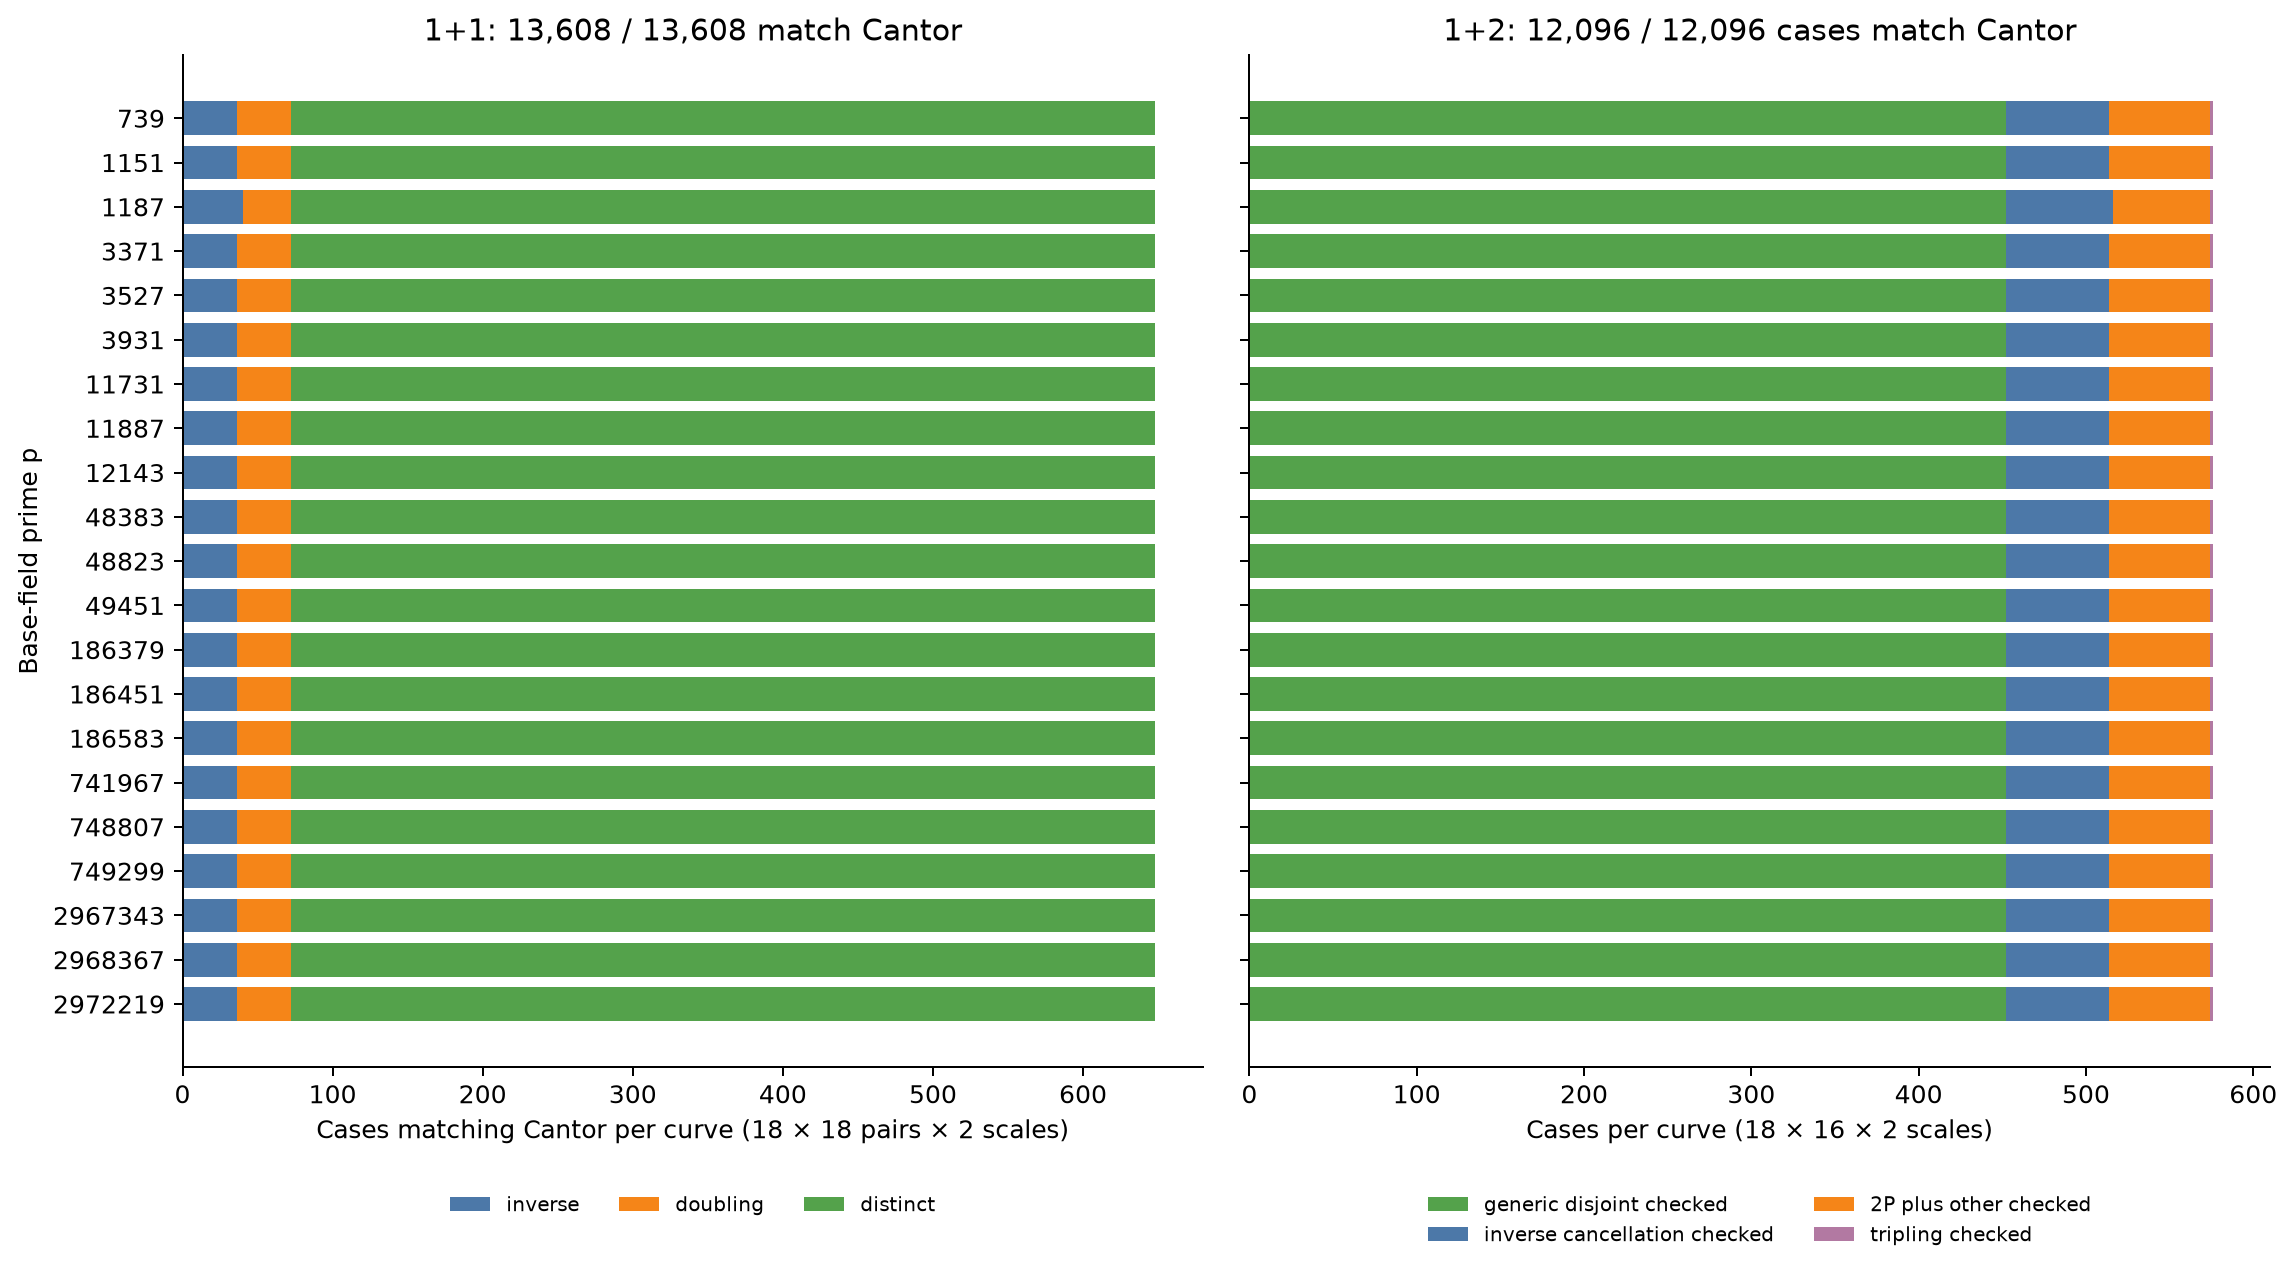
\includegraphics[width=0.98\linewidth]{complete-law-gate.png}
\end{center}
\begin{center}
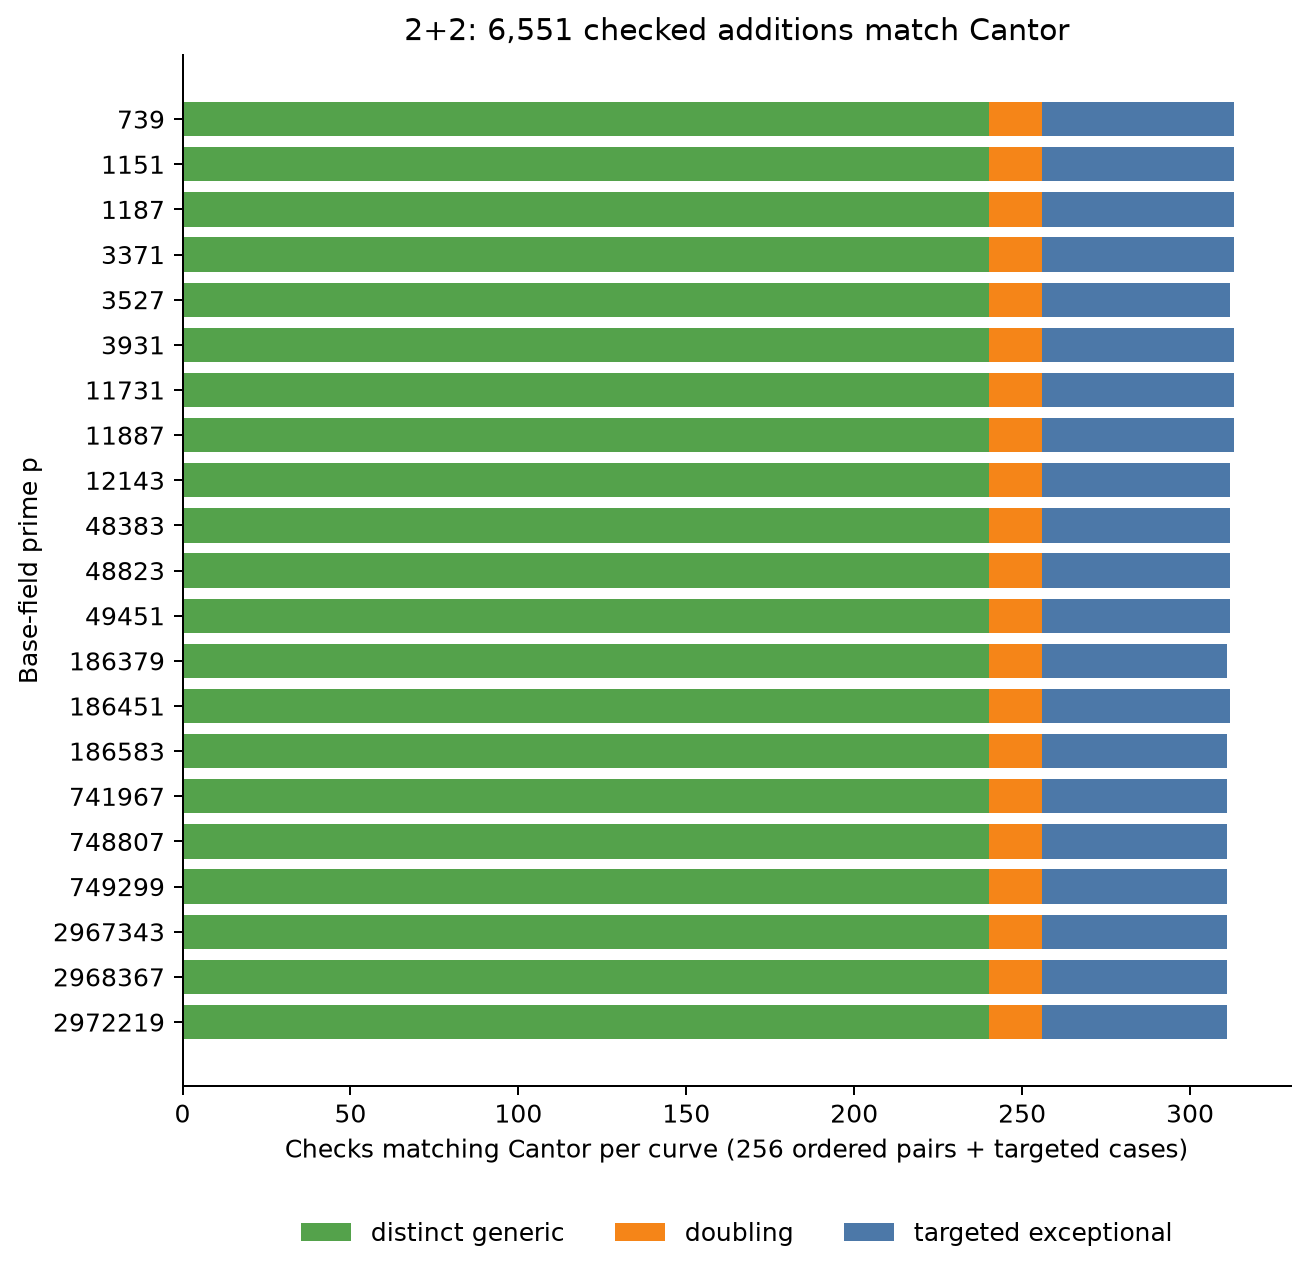
\includegraphics[width=0.72\linewidth]{complete-law-2plus2.png}
\end{center}
Raw records: \texttt{results/complete-law-branches.jsonl}. Source:
\texttt{src/bin/complete\_law\_gate.rs}. Arithmetic reference: Cantor
addition in the repository's independently developed Jacobian module.
\end{document}
